\documentclass[runningheads]{llncs}

\usepackage[utf8]{inputenc}
\usepackage[spanish,es-tabla]{babel}
\usepackage{amsmath,amssymb}
\usepackage{graphicx}
\usepackage{booktabs}
\usepackage{listings}
\usepackage{xcolor}
\usepackage{hyperref}


\lstset{
    language=Python,
    basicstyle=\ttfamily\scriptsize,
    keywordstyle=\color{blue}\bfseries,
    commentstyle=\color{gray}\itshape,
    stringstyle=\color{red!70!black},
    frame=single,
    breaklines=true,
    showstringspaces=false,
    numbers=left,
    numberstyle=\tiny\color{gray}
}

\begin{document}

\title{Implementación y Mejora de un Agente Aspiradora en un Entorno Bidimensional $3\times 3$ mediante Memoria de Estados y Métrica PEAS}
\titlerunning{Mejora del Agente Aspiradora $3\times 3$ con Memoria y PEAS}

\author{Lenin Amangandi\inst{1} \and Camila Caicedo\inst{1} \and Jarvin Ríos\inst{1}}
\authorrunning{Grupo DG\_2}

\institute{Escuela Politécnica Nacional, Facultad de Ingeniería de Sistemas,\\
Inteligencia Artificial (ICCD523), Quito, Ecuador\\
\email{lenin.amangandi@epn.edu.ec},
\email{camila.caicedo@epn.edu.ec},
\email{jarvin.rios@epn.edu.ec}\\
\url{https://github.com/Lenin27Amangandi/Inteligencia_Artificial_2k26.git}}

\maketitle

\begin{abstract}
En el presente informe técnico se analiza el desempeño de un agente reactivo simple aplicado al problema clásico del mundo de la aspiradora y se propone una mejora estructural escalada a una cuadrícula bidimensional de $3\times 3$. En primer lugar, se identifica la ineficiencia principal del agente reactivo aleatorio base, el cual decide únicamente en función de su percepción inmediata sin almacenar el historial de celdas visitadas ni contar con una condición de parada autónoma (\texttt{NoOp}), ocasionando un gasto energético continuo. Para resolver esta limitación, se diseña una métrica de rendimiento bajo el marco PEAS que recompensa la limpieza efectiva ($+10$ puntos) y penaliza el consumo energético por movimiento o aspirado ($-1$ punto). Posteriormente, se implementa un agente reactivo basado en modelos dotado de memoria y guiado por la distancia Manhattan hacia las celdas pendientes. La validación empírica sobre $50$ episodios demuestra que el agente mejorado incrementa el puntaje PEAS promedio de $10.40$ a $33.18$ puntos, reduce el consumo energético en un $56.6\%$ y alcanza el $100\%$ de limpieza frente al $46.0\%$ del agente aleatorio.

\keywords{Agentes Inteligentes \and Marco PEAS \and Agente Basado en Modelos \and Mundo de la Aspiradora \and Eficiencia Energética.}
\end{abstract}

\section{Introducción y Marco Teórico}

De acuerdo con Russell y Norvig \cite{russell2021}, un \textbf{agente} es cualquier entidad capaz de percibir su entorno a través de \textbf{sensores} y actuar sobre dicho entorno mediante \textbf{actuadores}. Matemáticamente, el comportamiento del agente se describe mediante la función de agente $f: P^* \rightarrow A$, la cual mapea cualquier secuencia de percepciones $P^*$ hacia una acción $a \in A$.

En el diseño de arquitecturas de agentes existen diferencias fundamentales según el uso de información histórica:
\begin{enumerate}
    \item \textbf{Agente Reactivo Simple:} Selecciona las acciones basándose únicamente en la percepción actual $p_t$, ignorando el resto del historial de percepciones. Funciona mediante reglas condición-acción (\textit{si estado = sucio entonces aspirar}), pero solo resulta óptimo si el entorno es completamente observable desde una única percepción \cite{russell2021}.
    \item \textbf{Agente Reactivo Basado en Modelos (con Memoria):} Cuando el agente solo percibe el estado local de la celda en la que se encuentra (observabilidad parcial), necesita mantener un \textbf{estado interno} (memoria) que registre qué partes del mundo ya han sido exploradas y limpiadas.
\end{enumerate}

\section{Especificación PEAS y Formalización del Problema}

Para evaluar objetivamente el comportamiento del agente en la cuadrícula escalada de $3\times 3$, se define la estructura \textbf{PEAS} (\textit{Performance, Environment, Actuators, Sensors}) en la Tabla~\ref{tab:peas}.

\begin{table}[htbp]
\centering
\caption{Definición del marco PEAS para el Agente Aspiradora en entorno $3\times 3$.}
\label{tab:peas}
\begin{tabular}{@{}p{3.2cm}p{8.5cm}@{}}
\toprule
\textbf{Componente PEAS} & \textbf{Descripción Técnica en el Simulador} \\ \midrule
\textbf{P}erformance (Rendimiento) & $+10$ puntos por cada celda sucia limpiada efectivamente; $-1$ punto de penalización energética por cada acción física (\texttt{Suck}, \texttt{Up}, \texttt{Down}, \texttt{Left}, \texttt{Right}); $0$ puntos de costo por detenerse (\texttt{NoOp}). \\ \addlinespace
\textbf{E}nvironment (Entorno) & Cuadrícula discreta bidimensional de $3\times 3$ ($9$ celdas), con estados de limpieza $\{0: \text{Limpio}, 1: \text{Sucio}\}$ generados aleatoriamente. \\ \addlinespace
\textbf{A}ctuators (Actuadores) & Mecanismo de aspirado (\texttt{Suck}), motores de desplazamiento en 4 direcciones (\texttt{Up}, \texttt{Down}, \texttt{Left}, \texttt{Right}) y apagado/reposo (\texttt{NoOp}). \\ \addlinespace
\textbf{S}ensors (Sensores) & Sensor de ubicación actual $(f, c) \in \{0,1,2\}^2$ y detector local de suciedad $s \in \{0, 1\}$. \\ \bottomrule
\end{tabular}
\end{table}

\subsection{Formalización Matemática del Problema de Búsqueda y Recorrido}
Siguiendo la formulación estándar de problemas en Inteligencia Artificial \cite{russell2021}, el entorno $3\times 3$ se define formalmente mediante los siguientes elementos:
\begin{itemize}
    \item \textbf{Espacio de estados ($S$):} Cada estado queda determinado por la posición del agente $(f, c) \in \{0,1,2\}^2$ y la matriz de estados de las $9$ celdas $G \in \{0,1\}^{3\times 3}$. El tamaño total del espacio de estados es $|S| = 9 \times 2^9 = 4\,608$ estados posibles.
    \item \textbf{Estado inicial ($s_0$):} Posición inicial $(f_0, c_0)$ aleatoria y configuración inicial de suciedad $G_0$ asignada de forma equiprobable.
    \item \textbf{Conjunto de acciones ($A$):} $A = \{\texttt{Suck}, \texttt{Up}, \texttt{Down}, \texttt{Left}, \texttt{Right}, \texttt{NoOp}\}$.
    \item \textbf{Prueba de meta ($Goal$):} Todas las celdas de la cuadrícula se encuentran limpias ($\sum_{i=0}^{2}\sum_{j=0}^{2} G_{i,j} = 0$) y el agente ha verificado las $9$ posiciones ($|\text{visitadas}| = 9$), ejecutando la acción terminal \texttt{NoOp}.
    \item \textbf{Costo de camino y Función de Rendimiento ($R$):} Cada acción física tiene un costo energético unitario $c(s, a, s') = 1$ (excepto $c(s, \texttt{NoOp}, s) = 0$). El puntaje PEAS total al finalizar un episodio de $T$ pasos se expresa como:
    \begin{equation}
        R = 10 \cdot N_{\text{limpiadas}} - \sum_{t=1}^{T} E(a_t), \quad \text{donde } E(a_t) = \begin{cases} 0 & \text{si } a_t = \texttt{NoOp} \\ 1 & \text{en otro caso} \end{cases}
    \end{equation}
\end{itemize}

\section{Identificación de la Ineficiencia y Diseño del Agente con Memoria}

\subsection{Ineficiencia del Agente Reactivo Simple Base}
Al ejecutar y analizar el código base proporcionado (\texttt{RandomVacuumAgent}), se identificaron dos fallas estructurales críticas:
\begin{enumerate}
    \item \textbf{Movimiento a ciegas sin memoria:} Cuando la celda actual está limpia, el agente escoge una dirección al azar (\texttt{random.choice}). Esto provoca que regrese repetidamente a celdas que ya limpió segundos antes, desperdiciando energía.
    \item \textbf{Ausencia de criterio de parada autónomo:} Como el agente solo conoce el estado de su celda actual y no guarda cuántas celdas ha revisado, nunca sabe si el resto de la habitación ya está limpia. Si no se detiene el ciclo externamente, el agente consume energía de forma infinita.
\end{enumerate}

\subsection{Arquitectura del Agente Mejorado (\texttt{MemoryVacuumAgent3x3})}
Para solucionar estas limitaciones de forma simple y eficiente, se implementó la clase \texttt{MemoryVacuumAgent3x3}, cuyo funcionamiento se resume en tres reglas:
\begin{enumerate}
    \item \textbf{Registro en memoria:} En cada paso, el agente almacena la coordenada actual $(f, c)$ dentro de una estructura de conjunto \texttt{self.visitadas}.
    \item \textbf{Limpieza prioritaria y parada óptima:} Si el sensor detecta suciedad ($s = 1$), retorna \texttt{Suck}. Si la celda está limpia y el conjunto \texttt{self.visitadas} ya contiene las $9$ celdas de la cuadrícula $3\times 3$, retorna \texttt{NoOp}, deteniéndose sin consumir más energía.
    \item \textbf{Selección de destino por Distancia Manhattan:} Si aún existen celdas no visitadas, el agente selecciona la celda pendiente $(f^*, c^*)$ más cercana empleando la heurística de distancia Manhattan. Dado que el entorno es una cuadrícula libre de obstáculos internos, esta métrica resulta ideal para calcular con exactitud el número mínimo de pasos de desplazamiento ortogonal necesarios:
    \begin{equation}
        d_M\big((f, c), (f', c')\big) = |f - f'| + |c - c'|
    \end{equation}
    y ejecuta un movimiento válido hacia dicha coordenada.
\end{enumerate}

\begin{lstlisting}[caption={Lógica principal del agente mejorado con memoria en Python.}]
class MemoryVacuumAgent3x3:
    def __init__(self):
        self.visitadas = set()
        self.todas_las_celdas = [(f, c) for f in range(3) for c in range(3)]

    def act(self, percept):
        pos, status = percept
        self.visitadas.add((pos[0], pos[1]))

        if status == 1:
            return 'Suck'

        celdas_pendientes = [c for c in self.todas_las_celdas if c not in self.visitadas]
        if len(celdas_pendientes) == 0:
            return 'NoOp'

        objetivo = min(celdas_pendientes, key=lambda c: abs(c[0]-pos[0]) + abs(c[1]-pos[1]))
        if objetivo[0] < pos[0]: return 'Up'
        if objetivo[0] > pos[0]: return 'Down'
        if objetivo[1] < pos[1]: return 'Left'
        return 'Right'
\end{lstlisting}


\section{Análisis Empírico (Benchmarking) y Resultados}

Para validar empíricamente la mejora lograda, se ejecutó el script \texttt{benchmark\_comparativo.py} evaluando tanto al agente aleatorio (\texttt{RandomVacuumAgent3x3}) como al agente con memoria (\texttt{MemoryVacuumAgent3x3}) sobre los mismos $50$ entornos aleatorios de tamaño $3\times 3$ (semilla fija \texttt{seed = 42}) durante un horizonte de $30$ pasos por episodio. Los resultados cuantitativos se presentan en la Tabla~\ref{tab:benchmark} y en la Figura~\ref{fig:benchmark}.

\begin{table}[htbp]
\centering
\caption{Comparación empírica promedio en $50$ episodios sobre cuadrícula $3\times 3$ ($30$ pasos máx.).}
\label{tab:benchmark}
\begin{tabular}{@{}lrr@{}}
\toprule
\textbf{Métrica de Evaluación} & \textbf{Agente Aleatorio ($3\times 3$)} & \textbf{Agente con Memoria ($3\times 3$)} \\ \midrule
Puntaje PEAS promedio (puntos) & $10.40$ & $\mathbf{33.18}$ \\
Energía consumida promedio (unidades) & $30.00$ & $\mathbf{13.02}$ \\
Episodios con limpieza al $100\%$ (\%) & $46.0\%$ & $\mathbf{100.0\%}$ \\
Tiempo de ejecución total ($50$ ep., ms) & $4.64\text{ ms}$ & $6.24\text{ ms}$ \\ \bottomrule
\end{tabular}
\end{table}

\begin{figure}[htbp]
    \centering
    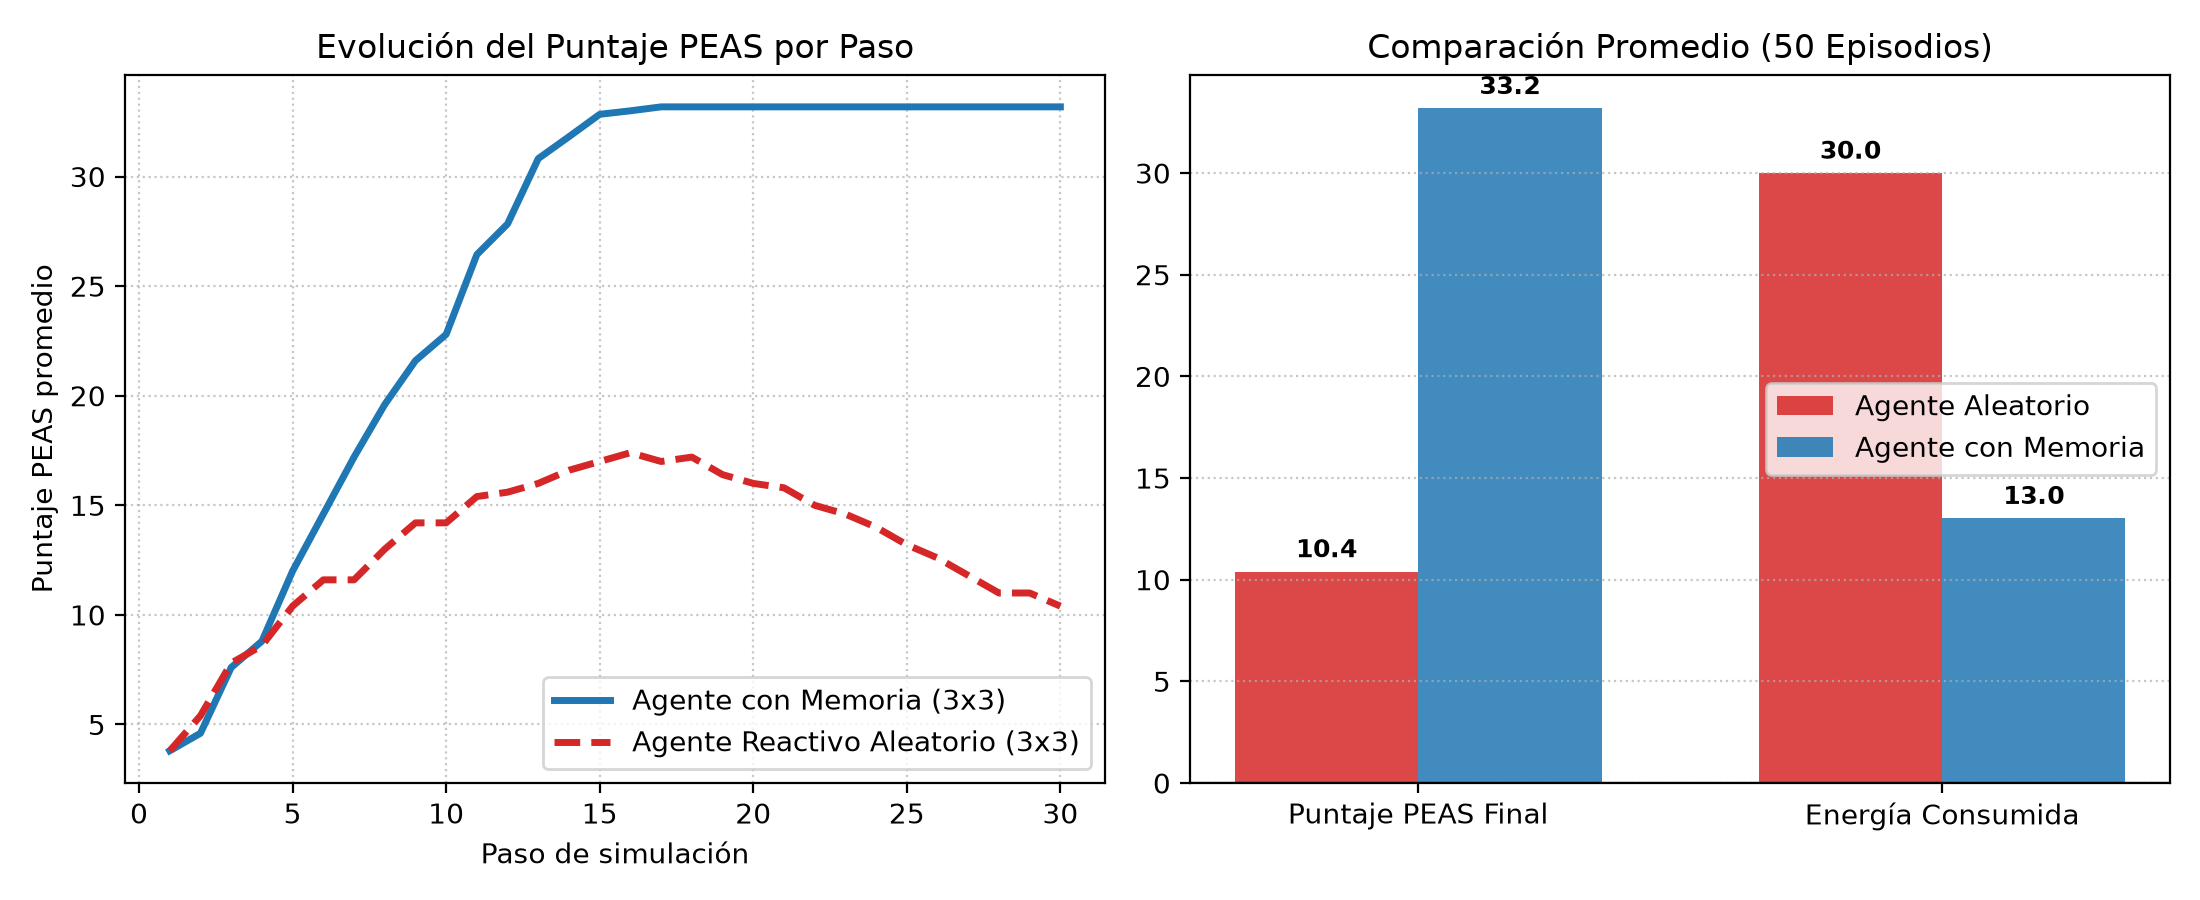
\includegraphics[width=0.98\textwidth]{comparacion_peas.png}
    \caption{Izquierda: Evolución paso a paso del puntaje PEAS promedio. Derecha: Comparación de puntaje final y energía consumida en 50 episodios.}
    \label{fig:benchmark}
\end{figure}


Como se observa en la Figura~\ref{fig:benchmark}, el agente aleatorio alcanza su pico de puntuación cerca del paso $10$, pero posteriormente su puntaje decae de manera lineal debido a que continúa desplazándose sin rumbo durante los $30$ pasos, consumiendo $30.00$ unidades de energía en promedio y dejando sucias celdas en el $54\%$ de los episodios. Por el contrario, el agente con memoria completa la exploración y limpieza de la cuadrícula $3\times 3$ en un promedio de $13.02$ acciones y se detiene con \texttt{NoOp}, manteniendo su puntuación máxima de $33.18$ puntos constante y logrando el $100\%$ de efectividad.

\section{Conclusiones, Trade-offs y Reflexión Ética}

\begin{enumerate}
    \item \textbf{Impacto del Estado Interno (Memoria):} La transición de un agente reactivo simple a un agente basado en modelos con memoria permitió triplicar el puntaje PEAS promedio, pasando de $10.40$ a $33.18$ puntos, además de garantizar la limpieza completa del entorno en la totalidad de los casos evaluados.
    \item \textbf{Evaluación de Trade-offs Computacionales:} Dotar de memoria al agente introduce un costo espacial lineal para almacenar las nueve coordenadas de la cuadrícula y un incremento mínimo en el tiempo de cómputo de $1.60\text{ ms}$ por el cálculo de la distancia Manhattan. Sin embargo, este costo es completamente despreciable frente al ahorro del $56.6\%$ en la energía física consumida por los actuadores.
    \item \textbf{Aplicaciones Reales y Reflexión Ética en IA:} En sistemas robóticos autónomos, como aspiradoras domésticas o drones de inspección, el desplazamiento sin rumbo degrada la batería y aumenta la huella de carbono. Desde la ética de la inteligencia artificial, integrar criterios claros de detención y planificación eficiente garantiza la sostenibilidad energética y evita que los agentes operen de manera errática tras cumplir su objetivo.
\end{enumerate}

\begin{thebibliography}{9}

\bibitem{russell2021}
Russell, S., Norvig, P.: Artificial Intelligence: A Modern Approach. 4th edn. Pearson, Hoboken, NJ (2021)

\bibitem{sutton2018}
Sutton, R.S., Barto, A.G.: Reinforcement Learning: An Introduction. 2nd edn. MIT Press, Cambridge, MA (2018)

\end{thebibliography}

\end{document}
